% ---------------------------------------------------------------
%  curl commit dd7521b.  Line numbers verified against
%  lib/transfer.c and lib/curl_ctype.h at that commit.
%  Panel (a) is wrapped in a save box and shrunk only if it would
%  overflow, so it can never run into panel (b).
%  In a two-column paper use figure* instead of figure.
% ---------------------------------------------------------------
\usetikzlibrary{positioning,arrows.meta,calc,shapes.geometric,shapes.misc,fit,backgrounds}
 
\definecolor{diffadd}{HTML}{CCEFCC}
\definecolor{diffaddtext}{HTML}{176117}
\definecolor{diffdel}{HTML}{F7D4D4}
\definecolor{diffdeltext}{HTML}{9B1111}
\definecolor{crashbg}{HTML}{FFE3B8}
\definecolor{crashfg}{HTML}{9A5300}
\definecolor{sizebg}{HTML}{E6E6E6}
\definecolor{sizefg}{HTML}{4A4A4A}
\definecolor{macrobg}{HTML}{E4E9F2}
\definecolor{macrofg}{HTML}{2E3F5C}
\definecolor{ctrlblue}{HTML}{15507F}
\definecolor{datapurple}{HTML}{6A3D9A}
 
\lstdefinestyle{pdgfig}{
  language=C, basicstyle=\ttfamily\scriptsize,
  keywordstyle=\color{black}, commentstyle=\color{black!45}\itshape,
  stringstyle=\color{black!70}, columns=fullflexible, keepspaces=true,
  showstringspaces=false, numbers=none, escapeinside={(*@}{@*)},
  xleftmargin=0pt, aboveskip=2pt, belowskip=2pt,
}
 
\tikzset{
  box/.style ={draw=black!60, rounded corners=2pt, fill=black!4,
               font=\scriptsize\ttfamily, align=center, inner sep=4pt,
               minimum height=7mm, text width=26mm},
  sml/.style ={box, text width=22mm},
  pred/.style={shape=chamfered rectangle, rounded corners=0pt,
               chamfered rectangle xsep=1em, chamfered rectangle angle=45},
  chg/.style ={box, draw=diffaddtext, line width=0.9pt, fill=diffadd},
  crs/.style ={box, draw=crashfg,     line width=0.9pt, fill=crashbg},
  siz/.style ={box, draw=sizefg, line width=0.8pt, fill=sizebg},
  mac/.style ={box, draw=macrofg, line width=0.8pt, fill=macrobg},
  src/.style ={box, draw=black!55, fill=white},
  phi/.style ={draw=black!60, fill=black!6, ellipse, inner sep=2pt,
               font=\scriptsize},
  cf/.style  ={-{Latex[length=1.8mm]}, ctrlblue, semithick},
  df/.style  ={-{Latex[length=1.8mm]}, datapurple, semithick,
               dash pattern=on 2.2pt off 1.8pt},
  fd/.style  ={-{Latex[length=2.4mm]}, crashfg, line width=1.1pt,
               dash pattern=on 3.5pt off 2pt},
  mx/.style  ={-{Latex[length=1.8mm]}, macrofg, dotted, thick},
  mis/.style ={{Latex[length=2.4mm]}-{Latex[length=2.4mm]}, crashfg,
               line width=1.1pt, dash pattern=on 3pt off 2pt},
  slice/.style={draw=black!70, line width=0.9pt, rounded corners=4pt,
               dash pattern=on 3pt off 1.6pt on 0.8pt off 1.6pt,
               fill=yellow!35, inner sep=2.6pt},
  lb/.style  ={font=\tiny\sffamily, inner sep=1.5pt, fill=white,
               fill opacity=0.9, text opacity=1},
}
 
% line-number label: smaller and quieter than the code it annotates
\newcommand{\lno}[1]{{\tiny\sffamily\textcolor{black!50}{#1}}}
\newsavebox{\pdgcode}
\newlength{\pdgw}
% width of the longest listing line (48 monospace chars) plus colorbox padding
\settowidth{\pdgw}{\ttfamily\scriptsize 123456789012345678901234567890123456789012345678}
\addtolength{\pdgw}{10pt}
 
% ---- panel (a) is measured first, then shrunk only if too wide ----
\begin{lrbox}{\pdgcode}
\begin{minipage}{\pdgw}
\begin{lstlisting}[style=pdgfig]
(*@\textcolor{black!45}{\itshape lib/curl\_ctype.h}@*)
  68(*@\colorbox{macrobg}{\texttt{~\#define ISPRINT(x) \textbackslash}}@*)
   (*@\colorbox{macrobg}{\texttt{~~(Curl\_isprint((int)((unsigned char)x)))}}@*)
 
(*@\textcolor{black!45}{\itshape lib/transfer.c -- strlen\_url(), unchanged}@*)
1477(*@\colorbox{sizebg}{\texttt{~~~if(*ptr >= 0x80)}}@*)
1478(*@\colorbox{sizebg}{\texttt{~~~~~newlen += 2;}}@*)
1479(*@\colorbox{sizebg}{\texttt{~~~newlen++;}}@*)
 
(*@\textcolor{black!45}{\itshape lib/transfer.c -- caller, unchanged}@*)
1780   newlen = strlen_url(newurl, FALSE);
1785   newest = malloc(newlen + 1);
1789   strcpy_url(newest, newurl, FALSE);
 
(*@\textcolor{black!45}{\itshape lib/transfer.c -- strcpy\_url(), changed}@*)
1500   char *optr = output;
1508   for(iptr = (unsigned char *)url;
1509       *iptr;
1510       iptr++) {
1517     switch(*iptr) {
1518     case '?': ...
1521     default:
1522(*@\colorbox{diffdel}{\textcolor{diffdeltext}{\texttt{-~~~~~~if(*iptr >= 0x80) \{}}}@*)
1522(*@\colorbox{diffadd}{\textcolor{diffaddtext}{\texttt{+~~~~~~if(!ISPRINT(*iptr)) \{}}}@*)
1523         snprintf(optr,4,"%%%02x",*iptr);
1524         optr += 3;
1525       }
1526       else
1527         *optr++=*iptr;
1528       break;
1529     case ' ': ...
1538     }
1539   }
1540(*@\colorbox{crashbg}{\texttt{~~*optr = 0;}}@*)
\end{lstlisting}
\end{minipage}
\end{lrbox}
 
\begin{figure}[tb]
\centering
\begin{minipage}[t]{0.44\linewidth}
\centering
{\footnotesize\textbf{(a) reference code (commit \texttt{dd7521b})}}\\[3pt]
\ifdim\wd\pdgcode>\linewidth
  \resizebox{\linewidth}{!}{\usebox{\pdgcode}}%
\else
  \usebox{\pdgcode}%
\fi
\vspace{3pt}
 
{\tiny\sffamily
 \colorbox{macrobg}{\vphantom{Ay}~~}~macro \;
 \colorbox{sizebg}{\vphantom{Ay}~~}~sizing \;
 \colorbox{diffdel}{\vphantom{Ay}~~}~removed \;
 \colorbox{diffadd}{\vphantom{Ay}~~}~added \;
 \colorbox{crashbg}{\vphantom{Ay}~~}~faulting}
\end{minipage}
\hfill
\begin{minipage}[t]{0.53\linewidth}
\centering
{\footnotesize\textbf{(b) control- and data-flow dependences}}\\[3pt]
\resizebox{\linewidth}{!}{%
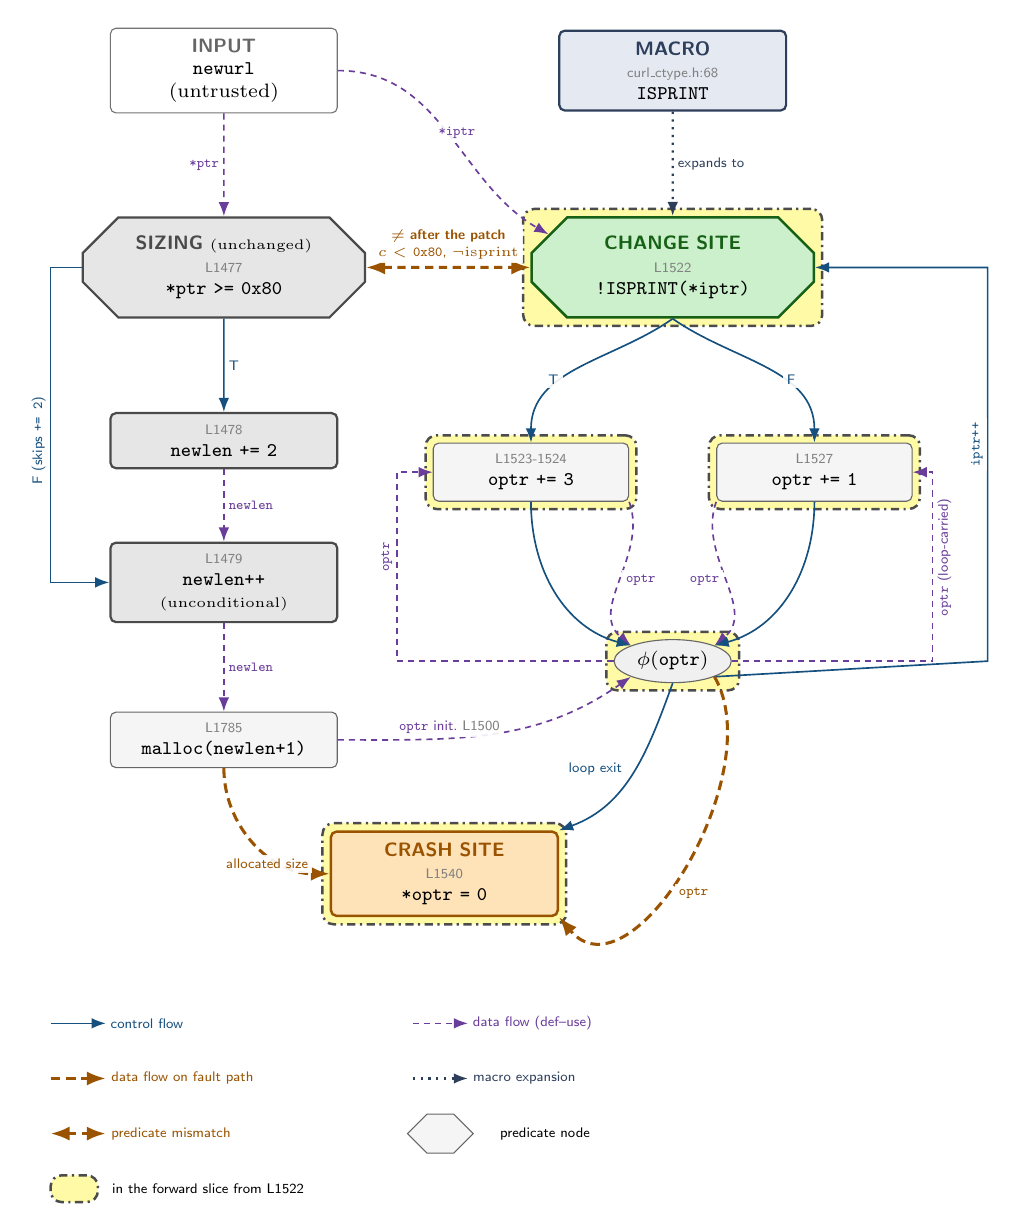
\begin{tikzpicture}
 
\node[src] (url) at (-3.1,2.5)
  {\textcolor{black!60}{\sffamily\bfseries INPUT}\\ \texttt{newurl}\\
   \textrm{\scriptsize(untrusted)}};
 
\node[mac] (mac) at (2.6,2.5)
  {\textcolor{macrofg}{\sffamily\bfseries MACRO}\\ \lno{curl\_ctype.h:68}\\ \texttt{ISPRINT}};
 
\node[siz,pred] (sizep) at (-3.1,0)
  {\textcolor{sizefg}{\sffamily\bfseries SIZING}~\textrm{\tiny(unchanged)}\\
   \lno{L1477}\\ \texttt{*ptr >= 0x80}};
 
\node[chg,pred] (writep) at (2.6,0)
  {\textcolor{diffaddtext}{\sffamily\bfseries CHANGE SITE}\\ \lno{L1522}\\
   \texttt{!ISPRINT(*iptr)}};
 
\node[siz] (sdefa) at (-3.1,-2.2) {\lno{L1478}\\ \texttt{newlen += 2}};
\node[siz] (sdefb) at (-3.1,-4.0)
  {\lno{L1479}\\ \texttt{newlen++}\\ \textrm{\tiny(unconditional)}};
 
\node[sml] (esc) at (0.8,-2.6) {\lno{L1523-1524}\\ \texttt{optr += 3}};
\node[sml] (cpy) at (4.4,-2.6) {\lno{L1527}\\ \texttt{optr += 1}};
 
\node[box] (alloc) at (-3.1,-6.0) {\lno{L1785}\\ \texttt{malloc(newlen+1)}};
 
\node[phi] (phi) at (2.6,-5.0) {$\phi(\texttt{optr})$};
 
\node[crs] (crash) at (-0.3,-7.7)
  {\textcolor{crashfg}{\sffamily\bfseries CRASH SITE}\\ \lno{L1540}\\ \texttt{*optr = 0}};
 
% ---- forward slice from the change site (background layer) ----
\begin{scope}[on background layer]
  \foreach \n in {writep,esc,cpy,phi,crash}{\node[slice, fit=(\n)]{};}
\end{scope}
 
% ---- data flow (def-use) ----
\draw[df] (url) -- node[lb,midway,left]{\texttt{*ptr}} (sizep);
\draw[df] (url.east) to[out=0,in=150]
      node[lb,pos=.55,above]{\texttt{*iptr}} (writep.north west);
\draw[df] (sdefa) -- node[lb,midway,right]{\texttt{newlen}} (sdefb);
\draw[df] (sdefb) -- node[lb,midway,right]{\texttt{newlen}} (alloc);
\draw[df] (alloc.east) to[out=0,in=215]
      node[lb,pos=.35,above]{\texttt{optr} init.\ \lno{L1500}} (phi.south west);
 
% optr defined at both branches, reaching the merge
\draw[df] (esc.south east) to[out=290,in=140]
      node[lb,pos=.5,right]{\texttt{optr}} (phi.north west);
\draw[df] (cpy.south west) to[out=250,in=40]
      node[lb,pos=.5,left]{\texttt{optr}} (phi.north east);
 
% loop-carried: merged value read again by both branches next iteration
\draw[df] (phi.west) -- (-0.9,-5.0) -- (-0.9,-2.6)
      node[lb,pos=.55,rotate=90,above]{\texttt{optr}} -- (esc.west);
\draw[df] (phi.east) -- (5.9,-5.0) -- (5.9,-2.6)
      node[lb,pos=.55,rotate=90,below]{\texttt{optr} (loop-carried)} -- (cpy.east);
 
% ---- macro expansion ----
\draw[mx] (mac) -- node[lb,midway,right]{expands to} (writep);
 
% ---- control flow ----
\draw[cf] (sizep) -- node[lb,midway,right]{T} (sdefa);
\draw[cf] (sizep.west) -- (-5.3,0) -- (-5.3,-4.0)
      node[lb,pos=.55,rotate=90,above]{F (skips \texttt{+= 2})} -- (sdefb.west);
\draw[cf] (writep.south) to[out=215,in=90] node[lb,pos=.6,left]{T} (esc.north);
\draw[cf] (writep.south) to[out=325,in=90] node[lb,pos=.6,right]{F} (cpy.north);
\draw[cf] (esc.south) to[out=270,in=165] (phi.north west);
\draw[cf] (cpy.south) to[out=270,in=15]  (phi.north east);
\draw[cf] (phi.south east) -- (6.6,-5.0) -- (6.6,0)
      node[lb,pos=.55,rotate=90,above]{\texttt{iptr++}} -- (writep.east);
\draw[cf] (phi.south) to[out=250,in=20]
      node[lb,pos=.55,above left]{loop exit} (crash.north east);
 
% ---- the two predicates no longer agree ----
\draw[mis] (sizep) -- node[lb,midway,above,align=center,yshift=1pt]
      {$\neq$ \textbf{after the patch}\\ $c<\texttt{0x80}$, $\neg\mathrm{isprint}$}
      (writep);
 
% ---- data flow along the fault path ----
\draw[fd] (alloc.south) to[out=270,in=180]
      node[lb,pos=.6,below]{allocated size} (crash.west);
\draw[fd] (phi.south east) to[out=300,in=310]
      node[lb,pos=.55,below right]{\texttt{optr}} (crash.south east);
 
\begin{scope}[shift={(-5.3,-9.6)}]
  \draw[cf] (0,0)    -- (0.7,0)    node[lb,right]{control flow};
  \draw[df] (4.6,0)  -- (5.3,0)    node[lb,right]{data flow (def--use)};
  \draw[fd] (0,-0.7) -- (0.7,-0.7) node[lb,right]{data flow on fault path};
  \draw[mx] (4.6,-0.7)--(5.3,-0.7) node[lb,right]{macro expansion};
  \draw[mis](0,-1.4) -- (0.7,-1.4) node[lb,right]{predicate mismatch};
  \node[pred, draw=black!60, fill=black!4, font=\tiny,
        inner sep=2pt, text width=4mm, align=center]
        at (4.95,-1.4) {\vphantom{Ay}};
  \node[lb,right] at (5.65,-1.4) {predicate node};
  \node[slice, minimum width=6mm, minimum height=3.4mm, inner sep=0pt]
        at (0.3,-2.1) {};
  \node[lb,right] at (0.72,-2.1) {in the forward slice from L1522};
\end{scope}
 
\end{tikzpicture}}
\end{minipage}
 
\caption{Illustration of a regression in curl that manifests outside the changed code.}
\label{fig:pdg}
\end{figure}